\documentclass{article}

\usepackage{amsmath, mathtools, amsthm}

\usepackage{graphicx}
\graphicspath{ {./images/george_orwell/} {./inglese/images/george_orwell/} }

\title{George Orwell}
\author{asdrubalini}
\date{\today}

\begin{document}
    \maketitle

    \section{Animal Farm: Characters}

    \subsection{Mr. Jones}
    Mr Jones is the human farmer working for the poorly-run Manor Farm. The character is an allegory for the Russian Tsar Nicholas II, which which was killed during the February Revolution of 1917 by the liberals and the Bolsheviks. Characterized by his drinking problem, he will be overwhelmed by the violent animal's revolution. He will eventually unsuccessfully return into the farm in an attempt to re-establish his totalitarian regime over the animals

    \subsection{Old Major}
    Old Major is an old pig that inspires the animal's revolution. Allegorically, he can be compared to Karl Marx which was one of the main creators of the communist ideology or Vladimir Lenin, the communist leader of the early Soviet Union. Once he died, he got his skull cut and put on display like Lenin's body was left in an indefinite repose.

    \subsection{Napoleon}
    Napoleon is a large pig, considered the Leader of the Animal Farm. Like Joseph Stalin, he doesn't talk much but has a reputation of taking action. Once he gained some authority over the farm, he becomes more and more violent, thus requiring him to have his bodyguards.
    Completely ignoring the principles of Animalism, as time goes on, he becomes like the humans he wanted to overthrow in all possible ways: he consumes the community food supplies without caring about others, he starts to abuse alcohol (but bans other from consuming it) and his controlled-economy plans miserably fails leading to more poverty and a waste of resources.

    \subsection{Snowball}
    Snowball is an intellectual pig which starts the revolution and is the main Animalism's designer. Unlike Napoleon, he is much smarter and has good intentions about his ideology, wanting to grant a good and equal life to each animal. He risks his life in the revolution and doesn't profit from the powers he got, always trying to improve everyone's conditions.

    He is eventually overthrown by Napoleon who starts a totalitarian regime, much like what happened to Leon Trotsky in the early USSR. Some elements can also be associated with Lenin.

    \subsection{Squealer}
    A small pig who serves as Napoleon helper and manages the Animalist propaganda. His great lexical skills allow him to convince the animals to believe and support the regime. He can be compared to Vyacheslav Molotov, who in the Soviet Union had a similar role.

    \subsection{Minimus}
    A pig who writes the national Animalism's anthems. Can be compared to Vladimir Mayakovsky.

    \subsection{Boxer}
    Boxer is an extremely strong and hard-working cart-horse. He is very gullible and can be considered Napoleon's slave, doing much of the farm's work and believing that his lord is always right, being convinced by the propaganda he was exposed to. At some point he got punished by Napoleon's dogs for going against the regime. After being injured, he was sold by Napoleon to a local knacker to buy himself some whisky. His death was falsified by Squealer's propaganda, making other animals believe that he died to defend the homeland. He was a Stakhanovite.

    \subsection{Clover}
    Clover is a caring female cart-horse who shows concern for Boxer's health, since he often put too much energy into his job without getting anything in return.
    Like Boxer, she is not too smart and eventually starts believing the propaganda.

    \subsection{Benjamin}
    Benjamin is an old donkey, one of the few that is able to read and considered one of the most bright. His cynicism results in him not doing anything against the regime, believing that life will go on badly as it has always done. It is thought that Benjamin is a reflection of the author's persona.

    \subsection{Moses}
    Moses is a raven and Mr. Jones's personal pet. At first he follows Mr. Jones into exile but he reappears several years later working as entertainer, working for Napoleon and telling about a wonderful place above the clouds where pool animals can rest forever. 
    He can be seen as a religious figure, and has an analogy with the Soviet Union, where Stalin resorted to Orthodox Church to resist the invasion from the nazis.

    \subsection{Mollie}
    Mollie is a self-centered equine who refuses to work and is eventually killed by the regime.

    \section{George Orwell}
    He was born as Eric Blair in 1903 as a son of a minor colonial official. He was educate in Ethon in England where he began to develop an interest in socialism and atheism. After college he started to work for the Indian Imperial Police, but he quickly returned to England because he hated working in Burma. He returned in Europe working as a dishwasher in Paris. This gave him the ability to write about his experience among the underprivileged.

    When the Spanish Civil War broke out between the Republican Government and the right wing Fascists, he went to Spain to fight for the Republicans. He then served in the Second World War while working as a journalist for the BBC.

    He wrote Animal Farm because he wanted people to know the truth about communist dictatorships and totalitarian regimes.

    He had a conflict between his middle-class education and his identification with the working-class. His writings are inspired by Dickens and talk about social themes, anti-totalitarianism and liberty.

    Totalitarianism is a form of government where the State has a major power, exercise an extremely high degree of control and regulation over both public and private life.

    He also the creator of Doublespeak, which is a way of communicating the truth in a way that it sounds better than it really is, using euphemism.

    \section{1984}
    Nineteen Eighty-Four is a dystopian novel where he talks about the life in a big totalitarian system in the country of Oceania. The book is set-up in the year 1984, in London, a city full of terror and constant control of the Big Brother.

    Oceania is huge and controlled by The Party, which is split in the Inner Party (1\% of the population) and the Outer Party (18\% of the population). Then there are the Proles (81\% of the population) who are the labour power and live in poverty. The Brotherhood is an underground organisation who opposes the Party.

    Anyone who opposes the system is punished by the party, which is also able to see everyone's home from their televisions. A new language is created by the party, "Newspeak", which is set to replace the older "Oldspeak". In the new language, some words are removed and other are replaced.

    The ministry of truth aims to change history to promote doublethink, a manipulation of the mind by making people accept contradictions.

    The protagonist of the novel is Winston Smith, who experience an alienation from the society and a rebellion aginst the party. Julia is Winston's lover, a 25 year old girl who is also a rebel.

    The novel's aim is to inform people, giving them an interpretation of reality.

    \subsection{The Political Compass}

    The political compass is a chart that can be used to describe a political ideology on two axes, based on economic and social ideas.

    \begin{center}
        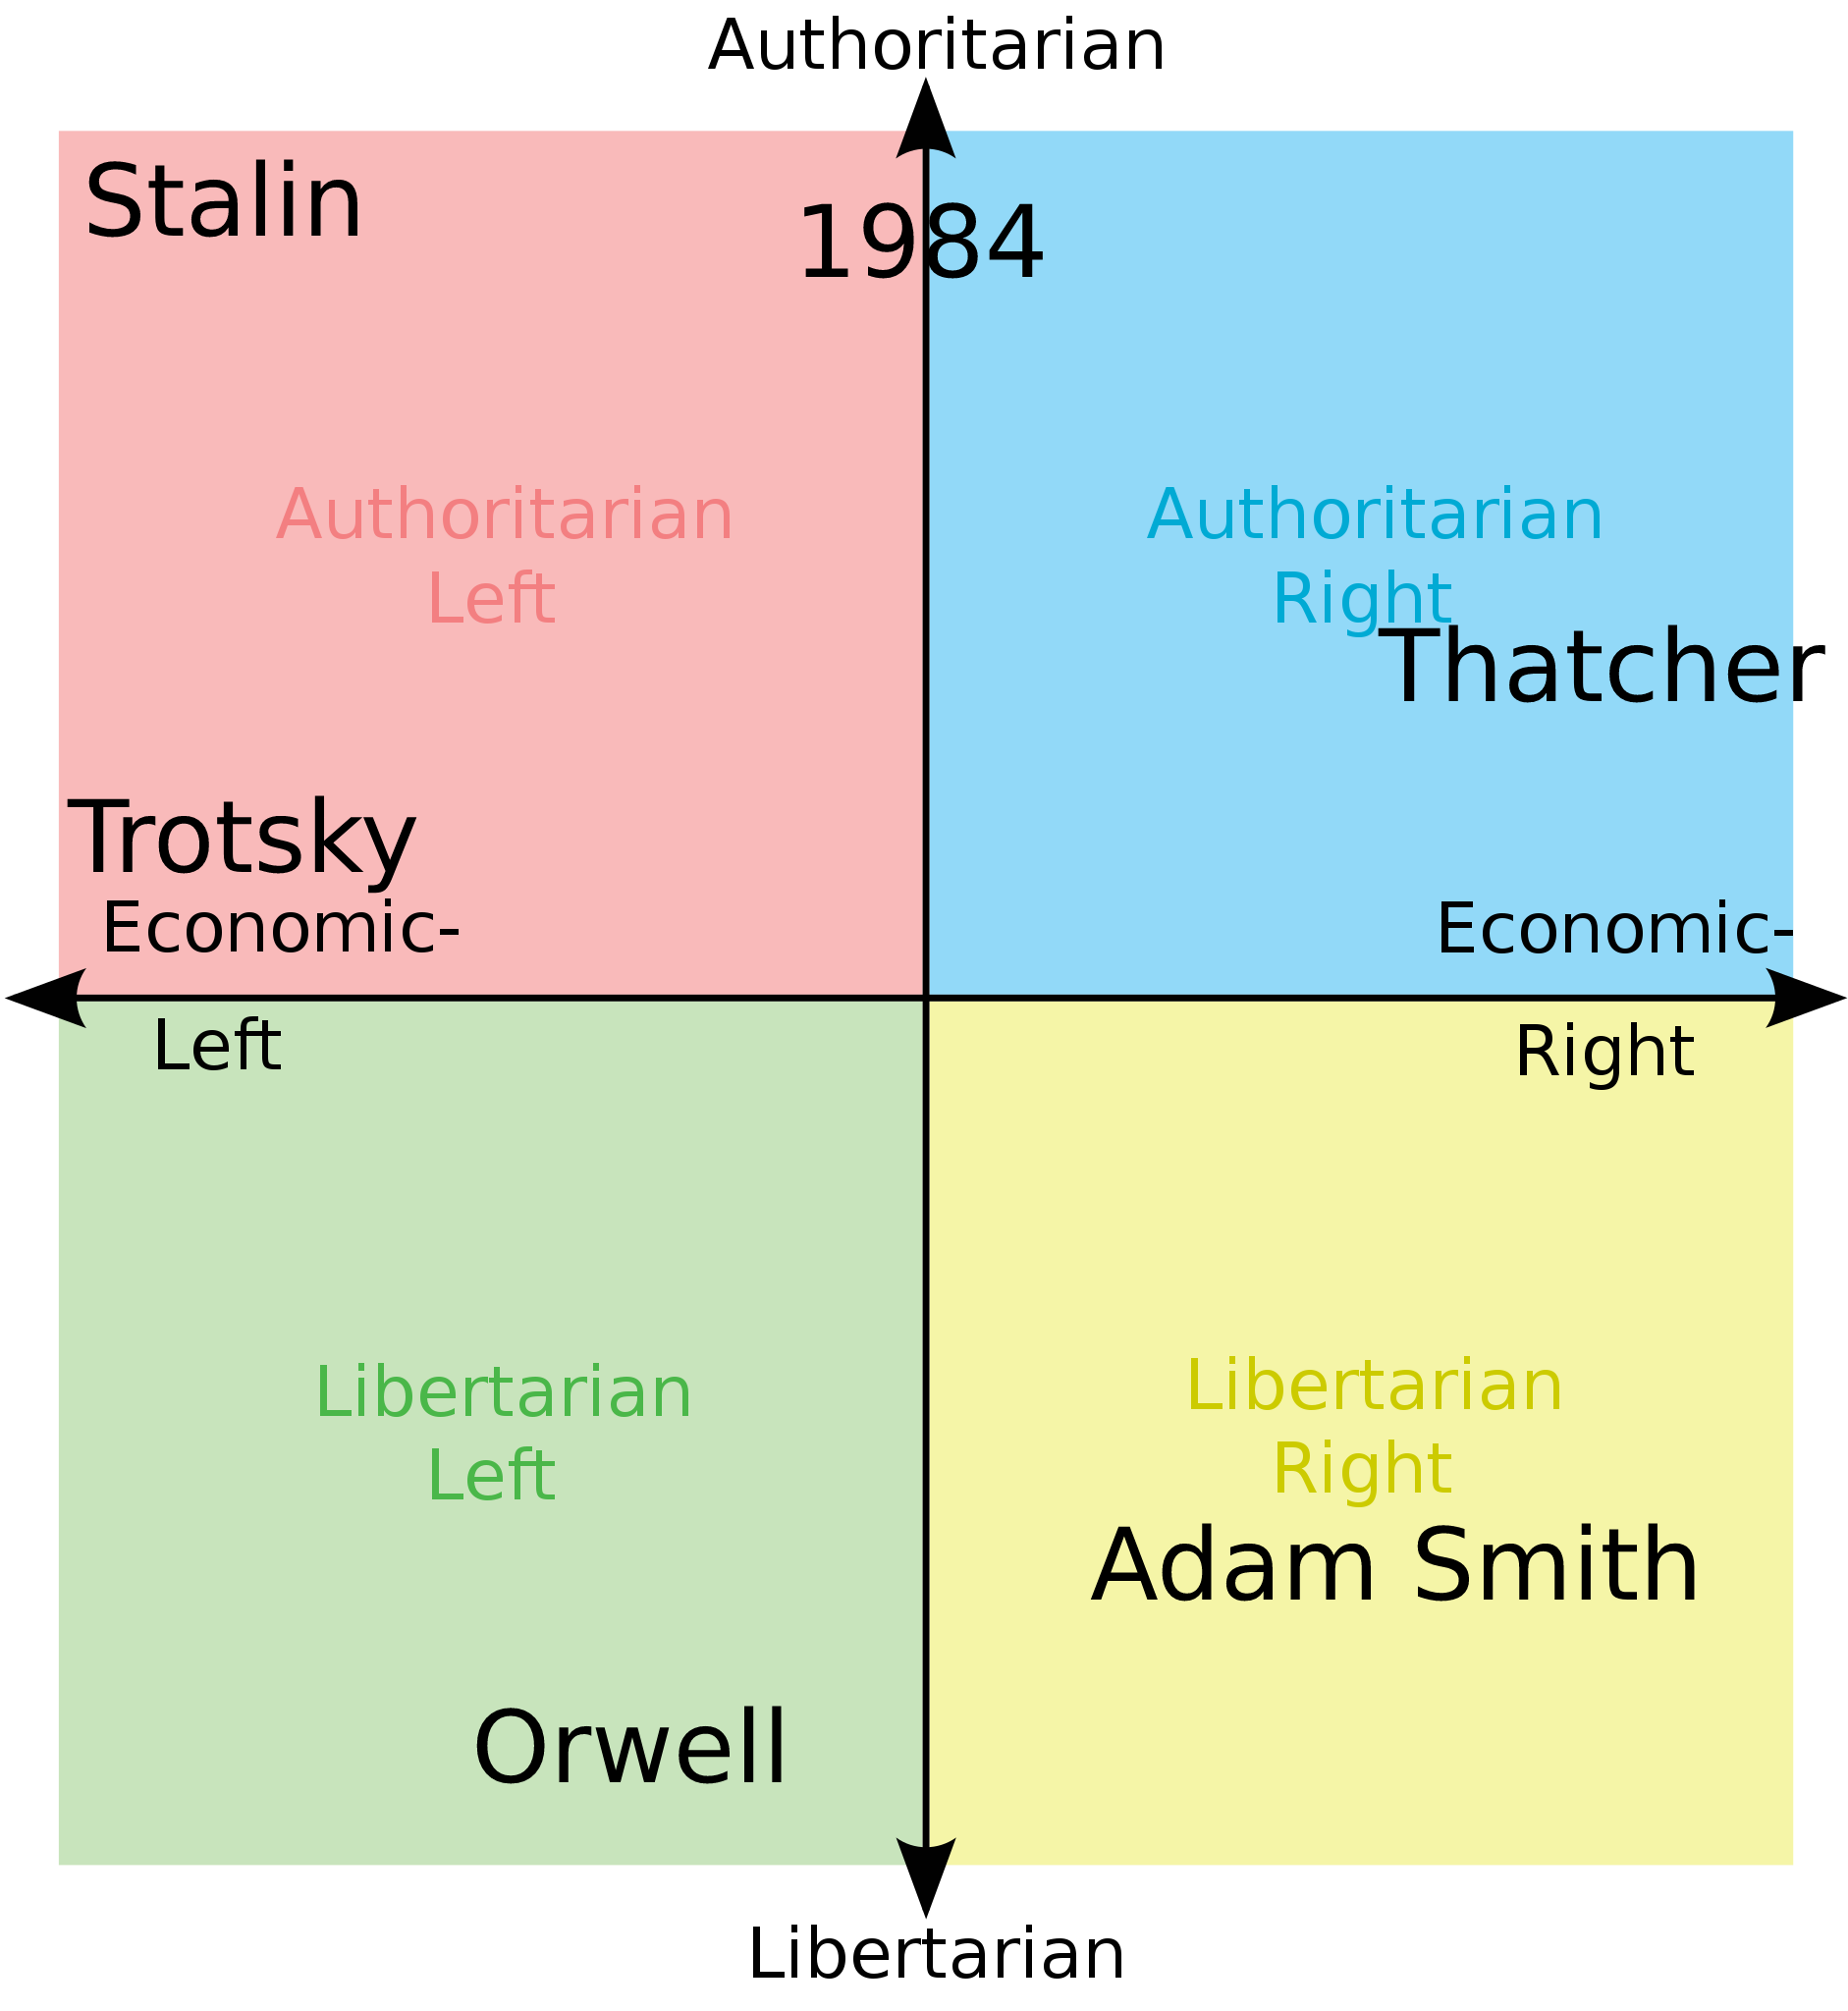
\includegraphics[width=\textwidth]{political_compass.png}
    \end{center}

    \section{Summary}
    \subsection{Chapter 1: The animals starts thinking of a rebellion}
    Mr. Jones, the human head of Manor Farm, has just gone to bed while forgetting to properly secure his farm buildings, when the animals joins together to hear a speech from Old Major, the pillar of the animal community, who is becoming older and older and is about to die.
    
    In his speech, he says that the lives of animals in the farm are miserable and comparable to the lives of slaves, while the land where they live would have enough resources to support many times the present population in luxury. He also blame humans as their oppressor, taking all the products of their labour and giving nothing in return.
    
    Old Major also share a dream he had, of a world where animals live free and happy without men. Animals have so much force compared to Mr. Jones that they could succeed in a rebellion if they joined their forces.

    \subsection{Chapter 2: The revolution is successful, and Animal Farm is born}
    Three days later, Old Major suddenly dies in his sleep, and the animals starts a preparation for their revolution that lasts 3 months.

    Napoleon and Snowball, two pigs, had the job to tech and organize the revolution. Together with Squealer and his speech abilities, they formulate the principles of what would become Animalism. At first, some animals had issues understanding the new ideology, since many of them would have to reject some of the luxiries they get from Mr. Jones.

    Moses starts spreading religious informations about a place where animals go once they die. The pigs work very had to convince others of the falsehood of Moses's teaching, but thanks to the help of two cart-horses, Boxer and Clover, the revolution begins.

    Mr. Jones, while drunk, forgets to feed the animals, so they break into a shed and begin to eat. Once Mr. Jones discovers this, he starts to whip the cows, which cause the animals to attack them, succeeding in the rebellion and conquering Manor Farm.

    The day after, the animals started going all around the farm discovering what they had never seen. They punished Mollie who tried to stay inside the house, and they declated that nobody could ever live in such a luxury, making Mr. Jones's house a museum.

    The farm is renamed to "Animal Farm" and the cows are milked by the pigs. Then, the animals go to the field in order to begin harvesting it, while Napoleon lags behind and drinks all the produced milk.

    \subsection{Chapter 3: Authority starts spreading across Animal Farm}
    The summer is spent harvesting the fields, and the total production exceeds any production the farm has ever seen. Everyone was working except Mollie and the cats who refused. Boxer in particular was working harder than everyone else, while Bejnamin didn't see any change under the new leadership.

    Animal Farm was being conducted under a democratic leadership, with a meeting every Sunday where new policies for the collective good were discussed.
    
    Snowball had some serious goal about the improvement of animals' lives, establishing some committees with various goals, and by the end of the summer, literacy rate increased for everyone.

    Even tough some animals could read, it became apparent that not everyone would be able to read and understand all the seven Commandments, so they got reduced to one main rule: “Four legs good, two legs bad.”.

    The animals got mad when they discovered that the pigs were eating all the apples and drinking all the milk, but Squealer quickly explained that the pig's brain need those to function properly and without, Mr. Jones could arrive.

    \subsection{Chapter 4: Mr. Jones is defeated once again by the animals}
    By the end of the summer, the news about Animal Farm starts spreading across the country, while Mr. Jones lives in Willingdon drinking all day. Animals everywhere beging singing and start with signs of rebellion.

    In October, some pidgeons alerts Animal Farm that Mr. Jones, together with other farmers, has begun marching towards the farm. Snowball, who has studied from books, prepare with the animals and they finally succeed in defeating the humans, with only a single death.

    Snowball and Boxer receive a medal while Mollie hid in order not to participate to the battle. October 12th was marked as the day of the victory with Mr. Jones's gun as the symbol.

    \subsection{Chapter 5: The expulsion of Snowball}
    Mollie is becoming a threat: she always arrives late at work, she didn't work hard and she often accepted threats from humans from near farms. She eventually disappears and is forgotten by the other animals.

    During the winder months, Snowball and Napoleon couldn't find an agreement on the future of the farm. Snowball wanted to build a windmill which could greatly improve animal's lifes, while Napoleon disagrees. When it comes time to vote, Napoleon use terror to scare the other animals inducing them to vote against Snowball's project. This would mark the end of the democracy in Animal Farm. Squealer would then explain that Napoleon is making a sacrifice in taking the leadership, and that Snowball was a traitor and a criminal, and that his expulsion from the farm is justified. The animals would accept this and Boxer adops two maxims: "I will work harder" and "Napoleon is always right".

    Three weeks after, it turns out that Napoleon supports the windmill project.

    \subsection{Chapter 6: The windmill is destroyed}

    The animals starts working hard for the construction of the windmill. By late summer, the construction starts. The animals works as hard as they used to do under Mr. Jones, and since the farm is running low on some resources, Napoleon hires a human solicitor, Mr. Whymper to assist him in trading. The pigs even started living in the farmhouse and sleeping in beds, even though one of the commandments disallow that. Squealer states that the commandment only disallows sleeping in beds with sheets.

    Around this time, a storm destroys the windmill, and Napoleon quickly says that it was sabotaged by Snowball, who would do anything he could in order to destroy Animal Farm.

    \subsection{Chapter 7: Food starts to be lacking and some animals get killed by Napoleon's police}
    During the winter, the animals starts rebuilding the windmill. In January they fall short of food, and the animals refuse to believe that the windmill fell because of Snowball, they instead think that the walls weren't thick enough.

    Napoleon agrees to sell 400 eggs a week, even though one of the original complaints was focused on the cruelty of egg selling.

    Squealer's propaganda convince the animals that Snowball was visiting the farm at night to sabotage their work, and Napoleon's dogs kill some animals that were forced to confess their participation in a conspiracy.

    Boxer starts working even harder, and a new song is composed by Minimus, the poet pig, which is then sung by the animals while working.

    \subsection{Chapter 8: The windmill is once again destroyed and the pigs starts to drink whisky}
    After the executions, the animals find out that the commandment reading “No animal shall kill any other animal” now reads: “No animal shall kill any other animal without cause.”, blaiming their memory for not remebering the final two words.

    Soon the construction for the windmill is done, but Napoleon discovers that the money given by Mr. Frederick is fake. A group of armed men starts attacking animal farm and with some dynamite the windmill gets destroyed. Boxer also gets seriously hurt.

    Some time later, the pigs discover a crate of whisky in the farmhouse and they start drinking like Mr. Jones used to do. The commandment saying that "No animal shall drink alcohol" is changed into "No animals shall drink alcohol to excess" by Squealer. Once again, the animals blame their memory.

    \subsection{Chapter 9: Boxer dies and Animal Farm becomes a republic}
    Boxer still works hard to rebuild the windmill, even if he is seriously injured. Food is even more scarce, while Squealer continues to say that the living conditions are better than those when there was Mr. Jones. A new motto was created, "Four legs good, two legs bad!"

    In April, Animal Farm is declared a republic and Napoleon becomes the president. Moses returns to the farm and once again begins spreading his stories about Sugarcandy Mountain. The pigs also allow him to live on the farm without working.

    One day, Boxer collapses while working. The pigs announce that he would be sent into a human hospital but he is instead being sent to a gluemaker to be slaughtered. Soon Squealer announces that the doctors could not cure him, and that he has died at the hospital. The pigs would then receive another crate of whisky.

    \subsection{Chapter 10: Pigs become humans}
    Years pass and the animals live a horrible life, except the pigs and dogs. The windmill is finished but is used for milling corn instead of generating electricity.

    One day, Squealer and Napoleon start walking on two legs. The wall with commandments now only read a phrase: "all animals are equal, but some animals are more equal than others".

    The pigs invite their human neighbour to visit the farm, and he appreciate the fact that the animals in Animal Farm work harder and with less food than any other animal. He also says that he would like to introduce the same business model into his own farm.

    Napoleon announces that the farm is going back to be called Manor Farm. The animals could not distinguish anymore who is the human and who is the pig.

\end{document}
